\documentclass[sigplan,screen,sigconf]{acmart}
\usepackage{minted}
\usepackage{fbox}
\settopmatter{printfolios=false,printacmref=false}
\bibliographystyle{ACM-Reference-Format}
\definecolor{bg}{rgb}{0.95,0.95,0.95}

\setcopyright{rightsretained}
\acmDOI{}
\acmISBN{}
\acmConference[LATTE '25]{Workshop on Languages, Tools, and Techniques for Accelerator Design}{March 30, 2025}{Rotterdam, Netherlands}

\author{Samit Basu}
\affiliation{
  basu.samit@gmail.com
  \country{Fremont CA, USA}
}

\begin{document}

\title{RHDL: Rust as a Hardware Description Language}

\begin{abstract}
In \cite{b13} proposed Rust as an excellent language for hardware description\footnote{FPGA Gateware or ASIC design}.  The initial attempt described in that paper was published as RustHDL \cite{b6}.  However, feedback from developers learning RustHDL revealed several weaknesses in the design.  As a result, I have developed RHDL \cite{b10}, which is a complete rewrite of RustHDL that attempts to address these shortcomings and significantly expand the capabilities of the tool.
\end{abstract}

\maketitle

\section{Introduction}

In my prior paper, I described the various reasons that Rust makes an excellent choice for a hardware description language.  This includes strong typing, functional programming features, package management and tooling, generics and a strong open ecosystem \cite{b0}, \cite{b9}. I also introduced RustHDL, which transforms a carefully selected subset of Rust into synthesizable Verilog.  Within a set of implicit rules, gateware can be built using Rust code.  There are, however, several shortcomings that became apparent as more engineers began to use RustHDL.  The complete list of feature requests is too long to list here, but includes:

\begin{itemize}
\item Algebraic Data Types (enums with data).
\item Type inference and local variable support.
\item Early returns, match and if expressions.
\item Timing estimation and analysis.
\end{itemize}

Adding these features has required the development of a co-compiler that runs alongside \verb|rustc| to analyze the Rust source code and generate a series of HDL-compatible representations that are successively lowered to the hardware. Both compilers work together to ensure that the language invariants are met at all stages, and that undefined behavior is prevented.  The new framework, called RHDL is meant to be a zero-cost abstraction, meaning that the framework itself does not limit the performance of the design.

\section{New Features}
RHDL (like it's predecessor RustHDL) is embedded in the Rust programming language, much as 
MyHDL is embedded in Python\cite{b3} and Chisel is embedded in Scala \cite{b2}.  As a result,
all RHDL code must be valid Rust and must meet all the requirements of the Rust compiler.  This design means an entire class of errors are eliminated, as the language enforces correct usage of types, prevents use-before-initialization, unassigned outputs, etc.  Furthermore, by using Rust itself, as opposed to something Rust-like or a DSL \footnote{Both Spade \cite{b1} and XLS \cite{b4} use a Rust-inspired syntax for hardware description.} all the tools that work with Rust can be used with RHDL unmodified.  Of course, the challenge with this approach is that only a very small set of Rust code can be directly mapped to Verilog.  Mapping a large subset of Rust to hardware requires significant analysis of the underlying code to enable the relevant transformations.  A brief summary of some of the more significant changes follows.

\subsection{Algebraic Data Types}
The main request from RustHDL users was support for Algebraic Data Types. These are essentially tagged unions, where the tag is created and tracked by the compiler, \emph{and it is guaranteed via the type system to be a valid combination of tag and data}.  This is an incredibly powerful feature in Rust that RustHDL was unable to support due to lack of any direct equivalent in Verilog.  RHDL provides first class support for ADTs. For example, the following can be used in synthesizable designs, where the language invariants guarantee that the payload is valid if and only if the appropriate tag is set in the discriminant of the enum:
\begin{minted}[fontsize=\footnotesize]{rust}
enum MyEnum {
  A, // No payload
  B(b4, b6), // 4-bit and 6-bit tuple payload
  C{ x: b4, y: b6, z: [b3; 3] }, // Struct payload
}
\end{minted}
All of these \emph{variants} are stored in a union that will be sized large enough to store the largest variant together with the discriminant.  In this case, the type is 21 bits wide.  See Figure~\ref{fig:my_enum} for an auto-generated layout diagram of the type.
\begin{figure}[H]
  \centering
  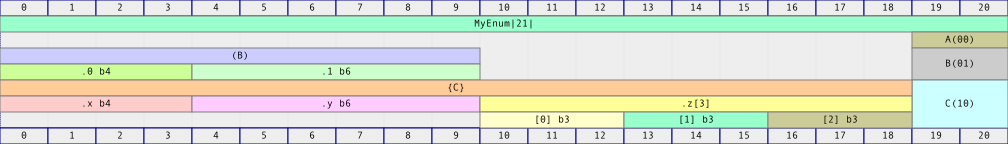
\includegraphics[width=8.5cm]{my_enum.png}
  \caption{Autogenerated layout of MyEnum.} \label{fig:my_enum}
\end{figure}


Using ADTs in Rust requires pattern matching and destructuring.  These are lowered into \verb|case| expressions automatically:
\begin{center}
\begin{minipage}{3.1cm}
\begin{minted}[fontsize=\footnotesize]{rust}
let w = MyEnum::B(1, 2);
let v = match w {
  MyEnum::A => bits(1),
  MyEnum::B(a,..) => a,
  MyEnum::C{ x,..} => x,
}
\end{minted}
\end{minipage}
$\rightarrow$
\begin{minipage}{4.1cm}
\begin{minted}[fontsize=\footnotesize]{rust}
let w = MyEnum::B(1, 2);
let a_if_w_is_B = __field(w,0); 
let x_if_w_is_C = __field(w,"x");
case __disc(w) {
  0 => y = bits::<4>(1),
  1 => y = a_if_w_is_B,
  2 => y = x_if_w_is_C,
}
\end{minted}
\end{minipage}
\end{center}
Note that this representation is notional - the actual compiler uses a different approach to transform the code, closer to a series of SSA opcodes.

\subsection{Type Inference and Local Variables}
Rust relies heavily on type inference to make the language less verbose.  RHDL uses a type inference pass to deduce and annotate the types of all variables in the original code.  This type pass \emph{must} agree with the types inferred by \verb|rustc| to avoid miscompilation.  Passes are included to ensure that all variables are typed by RHDL and that the typing is consisting with \verb|rustc|:
\begin{center}
\begin{minipage}{4cm}
\begin{minted}[fontsize=\footnotesize]{rust}
function(a: b4, b: b4) -> b4 {
  let x = 1;
  let y = (x, x + 1);
  y.0 + y.1
}
\end{minted}
\end{minipage}
$\rightarrow$
\begin{minipage}{3cm}
\begin{minted}[fontsize=\footnotesize]{rust}
  let a: b4;
  let b: b4;
  let x: b4;
  let y: (b4, b4);
  let _return: b4;
\end{minted}
\end{minipage}
\end{center}

Type inference and type checking are also used to enforce correctness of the design.  For example, in \verb|RHDL|, a \verb|Signal| type indicates the clock domain it belongs to by use of a parameter (designated via a color).  So, for example, \verb|Signal<b4, Red>| indicates a nibble that changes on edges in the \verb|Red| clock domain, and \verb|Signal<b4, Blue>| signifies a nibble that changes in the \verb|Blue| clock domain.   Here is an example that attempts to add signals from different clock domains (which is not allowed)
\begin{minted}[fontsize=\footnotesize]{rust}
function(a: Signal<b4, Red>, b: Signal<b4, Blue>) 
   -> (Signal<b4, Red>, Signal<b4, Blue>) {
  let a = a.val(); // Extract the value of a
  let b = b.val(); // Extract the value of b
  let a = a + b;   // <--- Illegal!
  (signal(a), signal(b))
}
\end{minted}
The user is presented with an error when attempting to compile this design:
\begin{figure}[H]
  \centering
  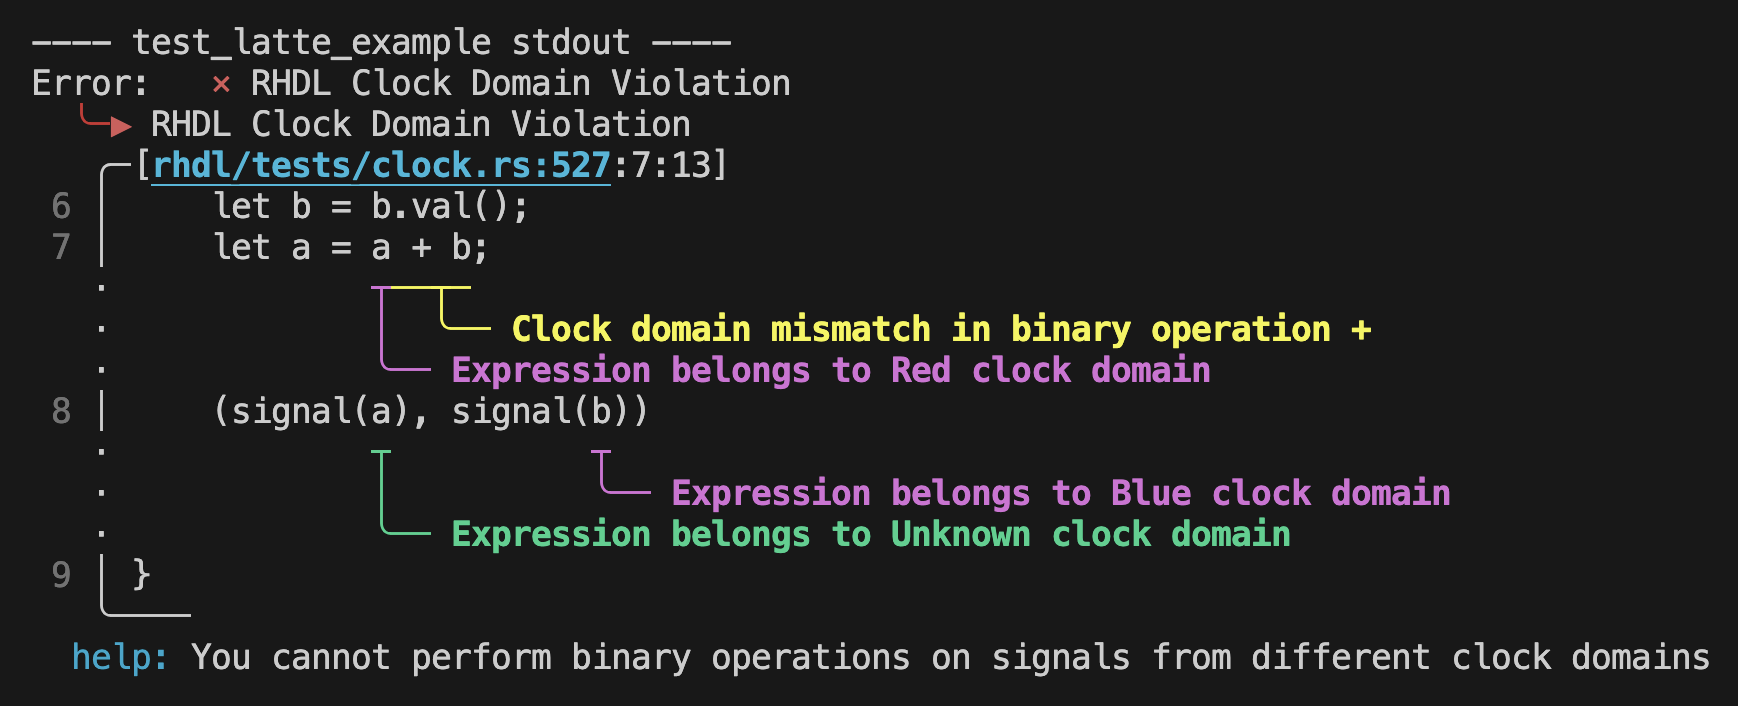
\includegraphics[width=6.5cm]{clock_error.png}
  \caption{Clock domain error message.}
\end{figure}
Clock domain crossings require special constructs that can safely cross signals from different clock domains.

\subsection{Expression Transformations}
Many Rust constructs are not directly mappable to Verilog.  For example, in Rust, all \verb|if| constructs are expressions, and can be used in any context where a value is expected.  Blocks also have values (in addition to side effects).  These are transformed into a series of mux expressions with renaming of local variables.

\begin{center}
  \begin{minipage}{0.25\linewidth}
    \begin{minted}[fontsize=\footnotesize]{rust}
let mut z = 0;
let x = if y {
  z += 1;
  z
} else {
  z
};
    \end{minted}
  \end{minipage}
    $\rightarrow$
    \begin{minipage}{0.57\linewidth}
  \begin{minted}[fontsize=\footnotesize]{rust}
let z = 0;
let z_if_y = z + 1;
let z_if_not_y = z;
let x = select(y, z_if_y, z_if_not_y);
let z = select(y, z_if_y, z_if_not_y);
  \end{minted}
\end{minipage}
\end{center}
Note that the mutable variable is also removed by renaming.  In this case, type inference will also be required as the types of all of the variables are implicit.  Similar transformations are applied for \verb|match| expressions, early returns and other flow control constructs.

\subsection{Timing Estimation}
A significant problem that arises in high level HDLs is the difficulty in fixing timing closure issues\footnote{Or any issues identified in downstream processing, such as floor planning, etc.} with the generated design.  This results from the very loose coupling between the design as expressed in the HDL and the resulting low level representation that feeds the synthesis tools.  RHDL includes a simple critical timing path estimator that can reference back to the source code:

\begin{figure}[h]
  \centering
  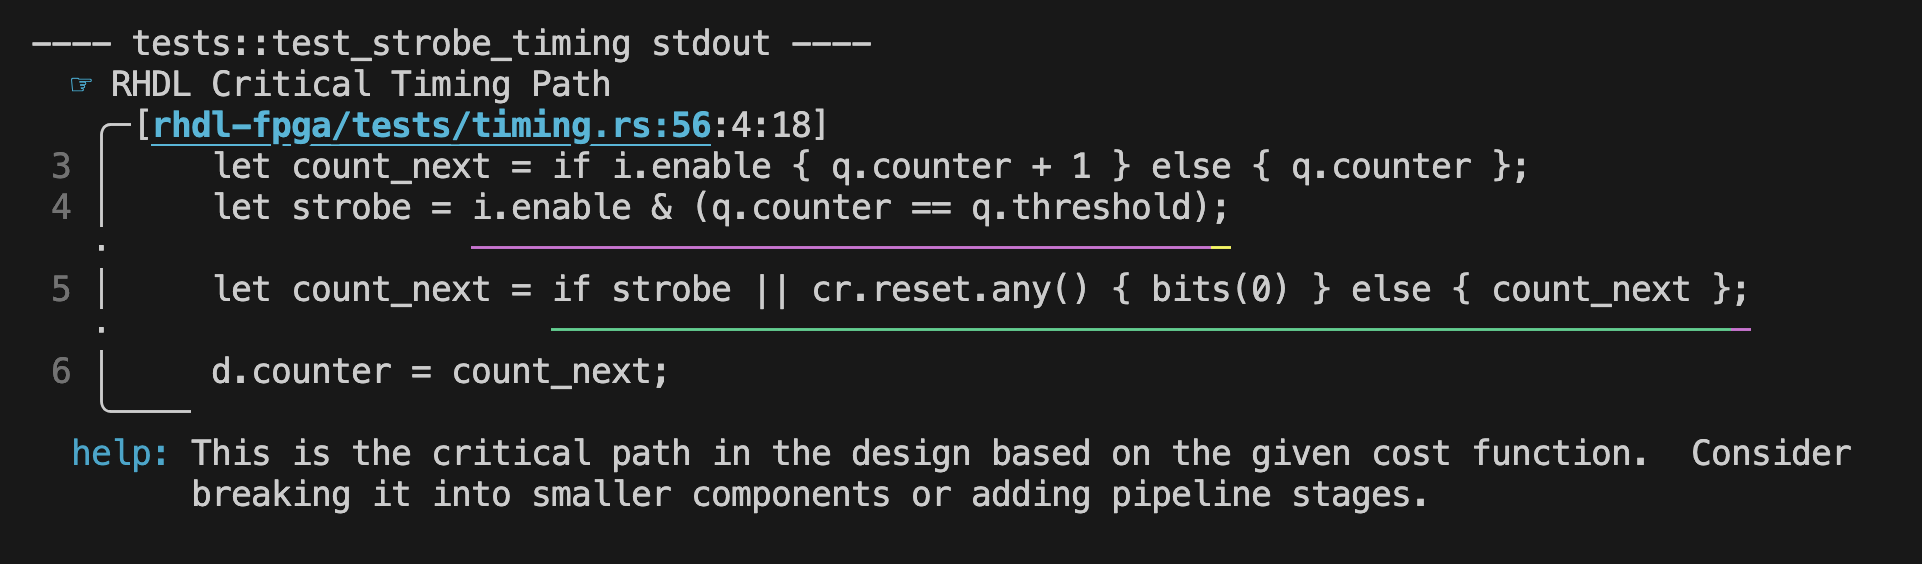
\includegraphics[width=6.5cm]{timing.png}
  \caption{Timing path estimation in RHDL}
\end{figure}

While basic, the intent is to build upon this capability to eventually include a closed loop from 3rd party tools back to the original source code.

\section{Internals}

RHDL requires a significantly more complex compiler than RustHDL.  RustHDL \cite{b13} is a transpiler, which generates Verilog syntax that is matched to the allowed subset of Rust that RustHDL supports, stripping type information out of the AST, and providing small shims to convert, e.g., \verb|match| statements into Verilog \verb|case| statements.  RHDL, on the other hand, requires a full compiler that treats Verilog more like a machine-code target than as a high level language.  The high level steps are:
\begin{itemize}
\item The AST is transformed to a Mid-level Intermediate Representation (MIR) which is typed static single assignment opcodes.
\item Type inference and lowering to RHDL Hardware Intermediate Form (RHIF).
\item RHIF is checked for type and clock domain issues, and optimized.
\item RHIF is lowered to an untyped RTL form after inlining.
\item RTL is further optimized and checked for correctness.
\item At this point, the module can be exported as Verilog for synthesis.
\item RTL is lowered into a flow graph representation (essentially a netlist).
\item Timing information is extracted from the flow graph.
\end{itemize}
In addition to these steps, the original code is compiled to a native binary by \verb|rustc|, and can be run using the built-in simulation engine to verify correctness of the design.  A few simple code annotations indicate what functions and structures are targets of synthesis.

\section{Conclusion}
RHDL is a significant step forward from RustHDL.  It enables the use of a more complete subset of Rust, and supports many more of the language features that make Rust a powerful language for software development.  These features should enable RHDL to support a wider range of hardware designs with code that is easier to write, correct, and efficient.

\newpage

\begin{thebibliography}{00}
  \bibitem{b13} S. Basu, ``Rust as a Hardware Description Language'', LATTE 2024, San Diego, CA.
  \bibitem{b6} ``RustHDL - Write FPGA Firmware using Rust!'', \url{https://rust-hdl.org/} (Accessed Feb 1, 2024).
  \bibitem{b10} ``RHDL - Rust Hardware Description Language'', \url{https://github.com/samitbasu/rhdl} (Accessed Jan 25, 2025).
  \bibitem{b0} ``Stack Overflow Developer Survey 2023'', \url{https://insights.stackoverflow.com/survey/2023} (Accessed Feb 1, 2024).
  \bibitem{b9} ``Rust - A language empowering everyone to build reliable and efficient software'', \url{https://rust-lang.org} (Accessed Feb 1, 2024).
  \bibitem{b3} ``MyHDL - From Python to Silicon!'', \url{https://www.myhdl.org/} (Accessed Feb 1, 2024).
  \bibitem{b2} ``Chisel - Software-defined hardware'', \url{https://www.chisel-lang.org/} (Accessed Feb 1, 2024).
  \bibitem{b1} F. Skarman and O. Gustafsson, ``Spade: An Expression-Based HDL With Pipelines'', Open Source Design Automation Conference, 2023.
  \bibitem{b4} ``XLS: Accelerated HW Synthesis'', \url{https://google.github.io/xls/} (Accessed Feb 1, 2024).
\end{thebibliography}
\end{document}
